\documentclass[reqno, oneside]{article}
\usepackage{style/preamble}
\usepackage{style/mytikz}
\usepackage{mathpazo}
\usepackage{parskip}
\setuptodonotes{disable}

\renewcommand*{\thefootnote}{\fnsymbol{footnote}}

\usepackage{fancyhdr}

\pagestyle{fancy}
\fancyhf{}
\rhead{Mathcamp 2019}
\lhead{Covering Spaces}
\cfoot{\thepage}

\usepackage{pgfplots}
\usepgfplotslibrary{polar}
\pgfplotsset{compat=newest}

\DeclareMathOperator{\Gal}{Gal}
\DeclareMathOperator{\groupaction}{\rotatebox{90}{$\circlearrowright$}}
\newcommand{\midarrow}{\tikz \draw[-triangle 90] (0,0) -- +(.1,0);}

\title{Galois Theory of Covering Spaces}
\author{\small{Apurva Nakade}}
\date{}

\begin{document}
  \cleardoublepage
  \pagenumbering{roman}
  \setcounter{tocdepth}{2}
  \maketitle
  \tableofcontents
  \cleardoublepage
  \pagenumbering{arabic}

  \maketitle
\section*{Motivation: Why covering spaces?}
\todo[inline]{Topologists have a love-hate relationship with topological spaces.}
One way to understand spaces is to associate an algebraic invariant to them.
\begin{equation*}
  \begin{tikzcd}
    \mbox{Topological Space} \ar[rr] && \mbox{Algebraic invariant} \\
    \mbox{For example: Knot} \ar[r] & \mbox{Knot projection} \ar[r] & \mbox{Knot invariant}
  \end{tikzcd}
\end{equation*}
where a knot invariant can be a number, polynomial, vector space, chain complex, etc.

It is rarely possible to compute an invariant directly using definition.
Instead, there are two main strategies in algebraic topology to compute these algebraic invariants:
\begin{enumerate}
  \item Break a space $X$ up into smaller spaces,
  \begin{align*}
    X = X_1 \cup \dots \cup X_n.
  \end{align*}
  This is called \emph{excision}.
  \item Map another space $Y$ into $X$ and recover information about $X$ using $Y$.
  \begin{align*}
    Y \longrightarrow X
  \end{align*}
  This is where covering spaces come in. A covering map $Y \rightarrow X$ provides us information about the fundamental group/first homotopy group $\pi_1(X)$.
  We will show later on that if $\pi_1(Y) \triangleleft \pi_1(X)$ then there is a short exact sequence of groups
  \begin{equation*}
    1 \rightarrow \pi_1(Y) \rightarrow \pi_1(X) \rightarrow \Gal(Y|X) \rightarrow 1
  \end{equation*}
\end{enumerate}

  \section{Introduction: Covering spaces}
A continuous map between spaces $p: Y \rightarrow X$ is a \emph{cover} or a \emph{covering map} if every point $x \in X$ has an open neighborhood $U$ such that \begin{enumerate}
  \item $p^{-1}(U)$ is a disjoint union of open sets $\sqcup_{i \in \cali} U_i$,
  \item $p$ restricted to each $U_i$ is an isomorphism.
\end{enumerate}
% \footnote{We'll later on show that the size of fiber does not depend on the point $x$.}
\begin{figure}[H]
  \centering
  \begin{tikzpicture}[scale=0.75]
   \draw [black,fill=gray!20] (0,0)  ellipse (2cm and 0.75cm);
   \draw [black,fill=gray!20] (0,1) ellipse (2cm and 0.75cm);
   \draw [black,fill=gray!20] (0,3.5) ellipse (2cm and 0.75cm);
    \node at (0,2.4) {$\vdots$};
   \node at (0, 0) {$\boldsymbol{\cdot}$};
   \node at (0, 1) {$\boldsymbol{\cdot}$};
   \node at (0, 3.5) {$\boldsymbol{\cdot}$};
   \draw (-4,0.5) -- (-4,0) -- (-2.25,0);
   \draw (-4,1.5) -- (-4,3.5) -- (-2.25,3.5);
   \node at (-4, 1) {$Y \supseteq p^{-1}(U)$};

   \draw [thick,->] (0,-1) -- (0,-3) node[midway,left] {$p$};

   \draw [black,fill=gray!20] (0,-4)
      ellipse (2cm and 0.75cm);
   \node at (-4, -4) {$X \supseteq U$};
   \node at (0, -4) {$\boldsymbol{\cdot}$};
   \node at (0.25, -4) {$x$};

\end{tikzpicture}

  \caption{Pancake picture of covering spaces}
\end{figure}
$U$ is said to be an \emph{evenly covered neighborhood}.
If $\abs{p^{-1}(x)} = k$ for ever $x \in X$, we say that $p$ is a $k$-cover.

\begin{ex}
  The most basic example of a covering space is
  \begin{equation*}
    I \rightarrow \{*\}
  \end{equation*}
  where $I$ is a discrete set.
  This is not very interesting, so from now on \textbf{we will assume that all our spaces connected.}
\end{ex}

\begin{ex}
  The only connected cover of $[0,1]$ is the space $[0,1]$ inself.
\end{ex}

\begin{ex}
  The first non-trivial example of a cover comes from a circle.
  \begin{align*}
    S^1 &\longrightarrow S^1 \\
    \theta \mod 2 \pi &\longmapsto n \theta \mod 2\pi
  \end{align*}
  The real line is also a cover of $S^1$.
  \begin{align*}
    \bbr^1 &\longrightarrow S^1 \\
    \theta &\longmapsto \theta \mod 2\pi
  \end{align*}
\end{ex}

\begin{ex}
  Turns out, the cylinder is a 2-covering of a mobius strip.
  It is hard to describe this using coordinates or equations, we'll instead do this combinatorially.
\end{ex}






\subsection{Spaces}
We will use cell complexes as a combinatorial model for spaces.
A \emph{2-cell complex} $X$ is a triple $(V, E, F)$ consisting of:
  \begin{enumerate}
    \item A non-empty set of vertices $V$.
    \item A set of directed edges $E$. For each edge $e \in E$, denote by $d_0 e$ and $d_1 e$ the starting and ending vertex of $e$ respectively. Denote by $e^{-1}$ the same edge but going in the opposite direction so that $d_0 e^{-1} = d_1 e$ and $d_1 e^{-1} = d_0 e$.
    \item A set of faces $F$.
  \end{enumerate}
  We further assume that our cell complexes are
  \begin{enumerate}
    \item \emph{locally finite} i.e. there are finitely many edges between any two vertices, and
    \item \emph{connected} i.e. there is a path of undirected edges connecting any two vertices.
  \end{enumerate}

A \emph{simplical map} between two cell complexes $p: X_0 \rightarrow X_1$ is a compatible triple of maps.
\begin{align*}
  V_0 \rightarrow V_1 && E_0 \rightarrow E_1 && F_0 \rightarrow F_1
\end{align*}
A simplical map is a covering space map if the induced map on the underlying topological spaces is one.

\begin{remark}
  Not every continuous map can be represented by a simplicial map, but every covering map can be. Further, there are more than one ways to describe a space using a graph.
\end{remark}






\subsubsection{Example: Covers of $S^1$}
For every integer $n$, there exists a unique $n$-cover of a circle.
  \begin{figure}[H]
  \centering
    \begin{tikzpicture}[thick]
      \begin{scope}[shift={(3,0)}, scale=0.5]
        \filldraw (0,0) circle (2pt);
\draw [->] (0,0) to [bend left=45] (1,1)  to [bend left=45] (2,0) node [right] {$a$};
\draw (2,0) to [bend left=45] (1,-1)  node [below] {$S^1$} to [bend left=45] (0,0);

      \end{scope}

      \draw [->] (-0.5,0) to node[midway, above] {$p$} (2.5,0);

      \begin{scope}[shift={(-3,0)}]
        \filldraw (0,0) circle (2pt);
\draw [->] (0,0) to [bend left=45] (1,1)  to [bend left=45] (2,0) node [right] {$a$};
\draw (2,0) to [bend left=45] (1,-1)  node [below] {$S^1$} to [bend left=45] (0,0);

      \end{scope}
    \end{tikzpicture}
    \caption{2-covering of a circle}
  \end{figure}
  Further, these covering maps form a poset: $nS^1$ is a cover of $mS^1$ if and only if $m$ divides $n$.
  $S^1$ has an infinite covering given by the real line.

  \begin{figure}[H]
  \centering
    \begin{tikzpicture}[thick]
      \begin{scope}[shift={(3,0)}, scale=0.5]
        \filldraw (0,0) circle (4pt);
        \draw [->] (0,0) to [bend left=45] (1,1) to [bend left=45] (2,0);
        \draw (2,0) to [bend left=45] (1,-1)  node [below] {$S^1$} to [bend left=45] (0,0);
      \end{scope}

      \draw [->] (-0.5,0) to node[midway, above] {$p$} (2.5,0);

      \begin{scope}[shift={(-5,0)}, scale=0.5]
        \filldraw (0,0) circle (4pt)
                  (2,0) circle (4pt)
                  (4,0) circle (4pt)
                  (6,0) circle (4pt);
        \draw [dashed] (-1,0) to (0,0);
        \draw [->] (0,0) to (1,0);
        \draw (1,0) to (2,0);
        \draw [->] (2,0) to (3,0);
        \draw (3,0) to node[midway, below] {$\bbr^1$} (4,0);
        \draw [->] (4,0) to (5,0);
        \draw (5,0) to (6,0);
        \draw [dashed] (6,0) to (7,0);
      \end{scope}
    \end{tikzpicture}
    \caption{Covering of $S^1$ by $\bbr^1$.}
  \end{figure}

  We will show that these covering spaces correspond to the subgroups of $\bbz$ and the inclusions of subgroups correspond to covering maps.
  \begin{align*}
    n \bbz &\longleftrightarrow nS^1 \\
    \set{0} &\longleftrightarrow \bbr^1 \\
    n \bbz \subseteq d \bbz &\longleftrightarrow nS^1 \rightarrow dS^1
  \end{align*}
  This is because the fundamental group of the circle is $\bbz$.


  \subsection{Example: $S^1 \vee S^1$}
  The space $S^1 \vee S^1$ (two circles glued at point) with 1 vertex, 2 edges, and 0 faces has very interesting covering spaces, see Figure \ref{fig:CoveringsOfS1S1}. The meanings of the various notations in Figure \ref{fig:CoveringsOfS1S1} will become clear later.
  \begin{figure}[H]
  \centering
    \begin{tikzpicture}[thick, scale=0.75]
      \filldraw (0,0) circle (2.5pt);

\draw [->] (0,0) to [bend right=45] (-1,1) to [bend right=45] (-2,0) node [left] {$a$} ;
\draw (-2,0) to [bend right=45] (-1,-1) to [bend right=45] (0,0);

\draw [->] (0,0) to [bend right=45] (1,-1) to [bend right=45] (2,0) node [right] {$b$};
\draw (2,0) to [bend right=45] (1,1) to [bend right=45] (0,0);

    \end{tikzpicture}
    \caption{$S^1 \vee S^1$}
  \end{figure}

  \begin{figure}[p]
  \centering
    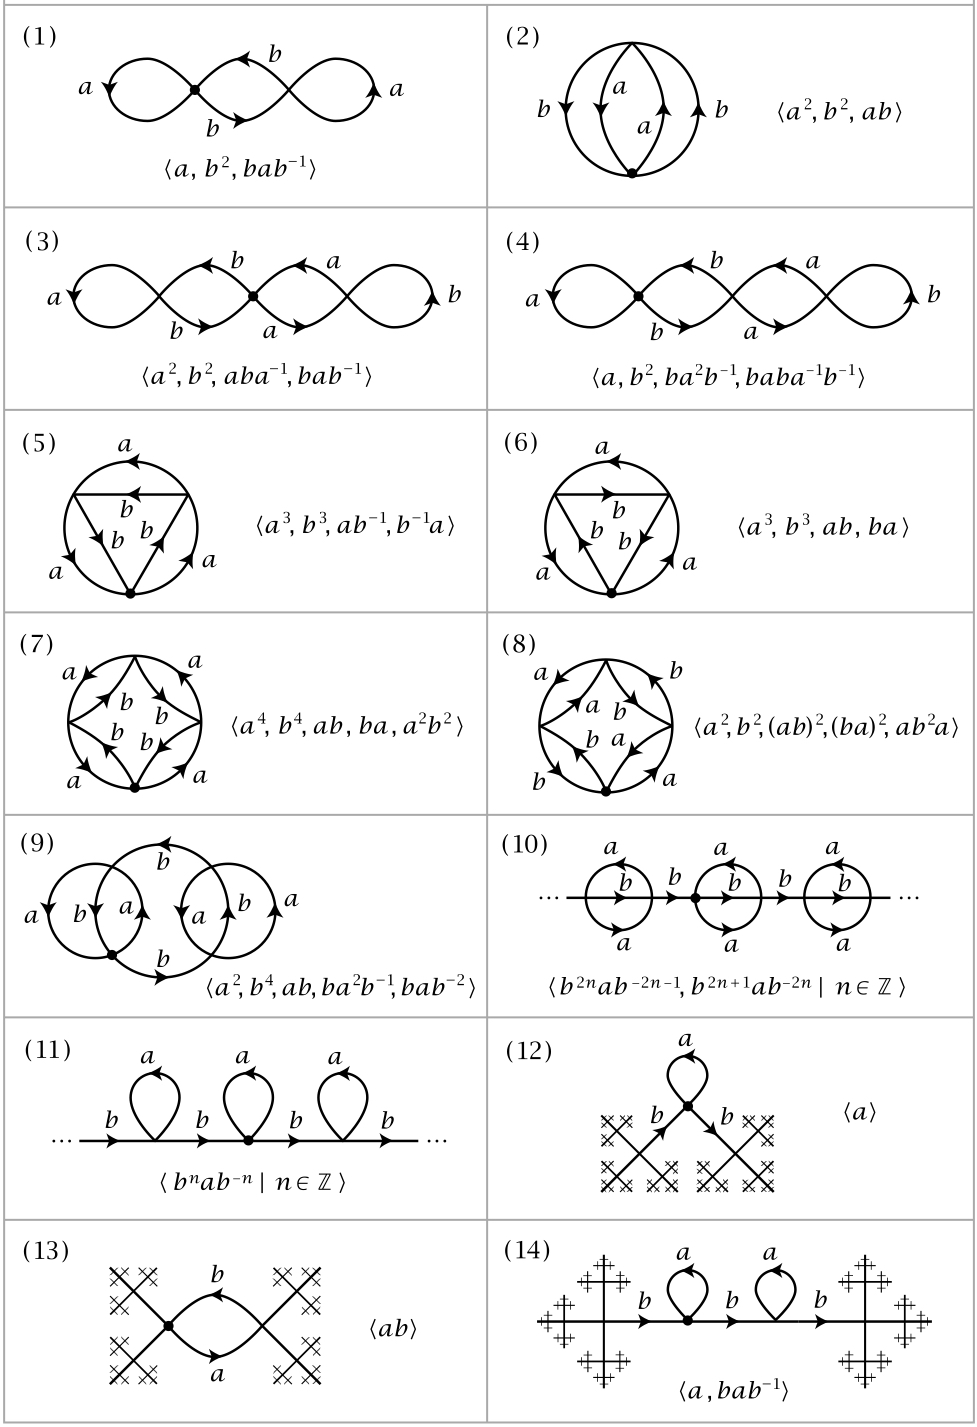
\includegraphics[width=\textwidth]{coveringsOfS1S1.jpg}
    \caption{Coverings of $S^1 \vee S^1$. Image from Algebraic Topology, Allen Hatcher, Chapter 1.}
    \label{fig:CoveringsOfS1S1}
  \end{figure}






  \subsubsection{Example: Gluing diagrams}
  We can form surfaces using 2-complexes, however these are harder to describe on paper.
  Instead, we use a trick called \emph{gluing diagrams}, Figure \ref{fig:GluingDiagrams}.
  These are ways to draw non-planar things on a plane, so there is some ambiguity and gluing going on in a gluing diagram that you should be careful about.

  \begin{qbox}
    In each of the gluing diagrams in Figure \ref{fig:GluingDiagrams}, count the number of vertices, edges, and faces.
  \end{qbox}

  \begin{qbox}
    Show that there are 2-cover maps
    \begin{align*}
      \mbox{Cylinder} &\longrightarrow \mbox{Mobius Strip} \\
      \mbox{Torus} &\longrightarrow \mbox{Klein Bottle} \\
      \mbox{Sphere } S^2 &\longrightarrow \mbox{Real projective space}
    \end{align*}
  \end{qbox}

  \begin{qbox}
    Guess the poset of covers of
    \begin{enumerate}
      \item Cylinder,
      \item Mobius Strip,
      \item Torus.
    \end{enumerate}
    Can you interpret these posets as subgroups of some groups?
  \end{qbox}


  \begin{figure}[p]
    \centering
    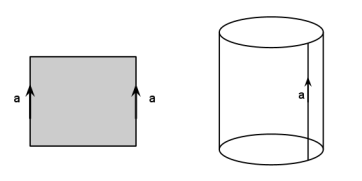
\includegraphics[width=0.8\textwidth]{cylinderGluingDiagram.png}
    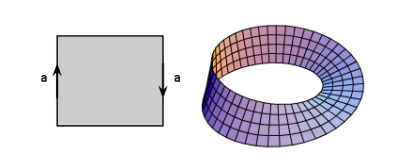
\includegraphics[width=0.8\textwidth]{MobiusStripGluingDiagram.png}

    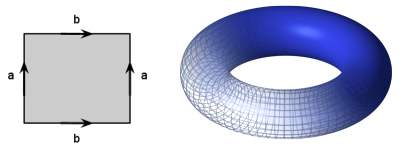
\includegraphics[width=0.8\textwidth]{torusGluingDiagram.png}
    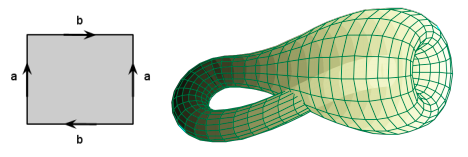
\includegraphics[width=0.8\textwidth]{KleinBottleGluingDiagram.png}

    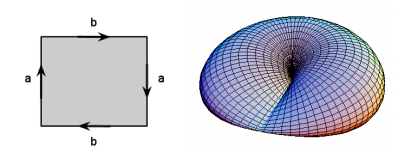
\includegraphics[width=0.8\textwidth]{RP2GluingDiagram.png}
    \caption{Gluing diagrams for cylinder, Mobius strip, torus, Klein bottle, real projective space respectively. Images from BMC Notes on Surfaces by Maia Averett.}
    \label{fig:GluingDiagrams}
  \end{figure}

  
% \section*{Why $S^1$ is a double cover of the Mobius strip.}
% \newpage
\section{Galois covers}
\label{sec:GaloisCovers}

We  will assume that all our maps are simplicial and all our group actions are via simplicial maps.
For a space $X$, denote by $X_0$, $X_1$, $X_2$ the vertices, edges, and faces of $X$.
All our spaces are connected and locally finite.

We can construct covering maps using group actions.
A left group action of a group  $G$ on a space $Y$, denoted $G \groupaction Y$, is a collection of simplicial maps
\begin{align*}
  g \cdot (-) : Y &\longrightarrow Y
\end{align*}
for $g \in G$ satisfying
\begin{enumerate}
  \item ${\mathbb{1}} \cdot (-) = \id$,
  \item $g \cdot (h \cdot (-)) = (gh) \cdot (-)$.
\end{enumerate}
\begin{qbox}
  Show that a group always acts via isomorphisms i.e. $g \cdot (-) : Y \rightarrow Y$ is an isomorphism.
\end{qbox}

\begin{definition}
  We say that the action of $G$ on $Y$ is \emph{free} if the induced group action on sets $Y_0$, $Y_1$, and $Y_2$ is free.
  The \emph{quotient space} $Y/G$ is the space with vertices, edges, and faces given by $Y_0/G$, $Y_1/G$, and $Y_2/G$ respectively.
\end{definition}

\begin{ex}
  If $d | n$ then the cyclic group $\bbz/d$ acts freely on $nS^1$ and the quotient space is precisely $(n/d)S^1$.
\end{ex}

\begin{qbox}
  Check that if $G \groupaction Y$ is free then $Y \rightarrow Y/G$ is a cover.\tablefootnote{For groups acting via continuous maps (and not simplicial maps) it is not true that $Y \rightarrow Y / G$ is always a covering space. We further require the group action to be \emph{properly discontinuous}. Fortunately, a group action via simplicial maps is always properly discontinuous.}
\end{qbox}
\begin{definition}
  We say that a cover $p:Y \rightarrow X$ is \emph{Galois} if there exists a left group action $G \groupaction Y$ such that $X \cong Y/G$.
\end{definition}
This definition is less that ideal as it relies on the existence of an abstract group $G$.
We will find an equivalent criterion for $p:Y \rightarrow X$ to be Galois which is completely intrinsic to the cover $p$.











\subsection{Paths and covers}
For the rest of Section \ref{sec:GaloisCovers}, fix a connected cover $p: Y \longrightarrow X$.

\begin{definition}
  For a vertex $x$ in $X$, $p^{-1}(x)$ is the \emph{fiber} over $x$.
\end{definition}



A \emph{path} of length $k$ in $X$ is a finite sequence of edges $\gamma = e_1 e_2 \dots e_k$, where we allow inverses, such that $d_1 e_i = d_0 e_{i+1}$ for $1 \le i \le k-1$.
Define $d_0 \gamma = d_0 e_1$ and $d_1 \gamma = d_1 e_k$.
Denote by $\gamma^{-1}$ the reverse path $e_k^{-1} \dots e_2^{-1} e_1^{-1}$.
% Two paths $\gamma_1, \gamma_2$ with $d_1 \gamma_1 = d_0 \gamma_2$ can be concatenated to get a path $\gamma_1 \cdot \gamma_2$ from $d_0 \gamma_1$ to $d_1 \gamma_2$.
% For $x \in X$, we'll denote by $\mathbb{1}_x$ the ``path of length 0'' at $x$.


  \begin{theorem}[Unique lifting of paths]
    \label{theorem:uniqueLiftingPaths}
    For every vertex $x$ in $X$, every path $\gamma$ in $X$ starting at $x$, and every vertex $y$ in the fiber $p^{-1}(x)$, there exists a unique path $\widetilde{\gamma}$ in $Y$ such that
    \begin{align*}
      \widetilde{\gamma} & \mbox{ starts at } y, \\
      p (\widetilde{\gamma}) &= \gamma.
    \end{align*}
    $\widetilde{\gamma}$ is called a \emph{lift} of $\gamma$.
  \end{theorem}

  \begin{qbox}
    Pick a path $\gamma$ of length 5 in $S^1 \vee S^1$.
    Draw lifts of $\gamma$ starting at the three different vertices in cover $(10)$ in Figure \ref{fig:CoveringsOfS1S1}.
  \end{qbox}

  \begin{proof}[Proof of Theorem \ref{theorem:uniqueLiftingPaths}]
    Proof is by induction on the length of $\gamma$.

    \emph{Base case: length of $\gamma = 1$.}
    Let $\gamma = e$ with $d_0 e = x$.
    Because $p$ is a covering map, there is a neighborhood of $x$ that is evenly covered. Hence, there is a unique edge (possibly an inverse) $\widetilde{e}$ with $d_0 \widetilde{e} = y$ and $p(\widetilde{e}) = e$. Then $\widetilde{\gamma} = \widetilde{e}$ is the required lift.
    \begin{qbox}
      Complete the induction step.
    \end{qbox}
  \end{proof}

    \begin{corollary}
      \label{corollary:surjectivityOfCovers}
      $p:Y \rightarrow X$ is surjective.
    \end{corollary}
    \begin{qbox}
      Prove that $p:Y_0 \rightarrow X_0$ is surjective by lifting appropriate paths. (Optional: Extend this proof to edges and faces.)
    \end{qbox}
    \begin{corollary}
      \label{corollary:cardinalityOfFibers}
      Every path $\gamma$ from $x_0$ to $x_1$ in $X$ naturally defines a bijection
      \begin{align*}
        p^{-1}(x_0) \longrightarrow p^{-1}(x_1).
      \end{align*}
      Hence, the fibers over any two vertices $x_0$, $x_1 \in X_0$, have the same cardinality.
    \end{corollary}
    \begin{qbox}
      Prove Corollary \ref{corollary:cardinalityOfFibers} using the lift of an appropriate path and it's inverse.
    \end{qbox}













\subsection{Deck transformations}
% Our goal is to come up with a criterion for $p$ being Galois.
% There is a very intricate relation between covering spaces and paths in the base space.




\begin{definition}
  A \emph{deck transformation} of $p$ is a simplicial map $\varphi: X \rightarrow X$ that commutes with $p$ i.e. $p = p \circ \varphi$.
  \begin{equation*}
    \begin{tikzcd}
      Y \ar[rr, "\varphi"] \ar[rd, "p"'] & & Y \ar[ld,"p"] \\
      & X
    \end{tikzcd}
  \end{equation*}
\end{definition}

\begin{qbox}
  Show that deck transformations of $p$ form a group.
\end{qbox}
Let $\Gal(Y|X)$ denote the group of deck transformations of $p: Y \rightarrow X$.
There is a natural left action of the group $\Gal(Y|X)$ on the space $Y$.

\begin{ex}
  For example, the Galois groups of the covers $(1)$, $(3)$, $(5)$ of $S^1 \vee S^1$ in Figure \ref{fig:CoveringsOfS1S1} are $\bbz/2$, $\set{\mathbb{1}}$, $\bbz/3$ respectively.
\end{ex}


\begin{qbox}
  Find the group of deck transformations of the covers $(2)$, $(6)$, $(7)$, $(8)$, $(9)$, $(10)$, $(11)$ of $S^1 \vee S^1$ in Figure \ref{fig:CoveringsOfS1S1}.
  For each of these covers $Y$, find quotient $Y / G$ where $G=\Gal(Y| S^1 \vee S^1)$.
\end{qbox}

\begin{qbox}
  Prov that for any vertex $x \in X$ and every deck transformation $\varphi \in \Gal(Y|X)$, we have $\varphi(p^{-1}(x)) = p^{-1}(x)$.
  Hence, the deck transformations permute the fibers over $x$.\tablefootnote{
  One can think of this as shuffling a deck of cards, hence the name ``deck'' transformations.}
\end{qbox}

% \begin{ex}
%   If $G \groupaction X$ freely then every element $ g \in G$ defines a decktransformation of $p: X \rightarrow G \backslash X$.
% \end{ex}

\begin{theorem}
  \label{theorem:freenessGaloisAction}
  The action of $\Gal(Y|X)$ on $Y$ is free.
\end{theorem}
\begin{proof}
  We will show that if a deck transformation $\varphi \in \Gal(Y|X)$ does not act freely on $ Y$, then $\varphi$ fixes everything and hence is the identity element in $\Gal(Y|X)$.

  Suppose the action of $\varphi$ is not free. It suffices to assume that $g$ fixes some vertex, as if $\varphi$ fixes some edge or a face then it also fixes the vertices of the edge or the face respectively. Suppose $\varphi y_0 = y_0$ for $y_0 \in Y$.

  Consider another vertex $y$ in $Y$. Let $x_0 = p(y_0)$ and $x = p(y)$.
  \begin{qbox}
    Using a path $\gamma$ in $Y$ from $y_0$ to $y$ show that $\varphi$ fixes $y$, thereby completing the proof of the proposition.
  \end{qbox}
\end{proof}


\begin{corollary}
  \label{cor:deckTransforms}
  Let $y$ be a vertex in $Y$ and let $\varphi, \varphi' \in \Gal(Y|X)$ be two deck transformations. If $\varphi(y) = \varphi'(y)$ then $\varphi = \varphi'$. Hence, a deck transformation is completely determined by where it sends one vertex!
\end{corollary}
\begin{qbox}
  Prove this.\hint{Look at $\varphi^{-1} \circ \varphi'$.}
\end{qbox}

\begin{theorem}
  \label{theorem:GaloisCriterion}
  A cover $p:Y \rightarrow X$ is Galois if and only if $\Gal(Y|X)$ acts freely, transitively on each of the sets $p^{-1}(x)$ where $x$ is a vertex, an edge, or a face in $X$.
\end{theorem}
\begin{proof}
  This is equivalent to showing that $p:Y \rightarrow X$ is Galois if and only if for any two $y_1$, $y_2 \in p^{-1}(x)$ there is a unique deck transformation $g \in \Gal(Y|X)$ such that $g \cdot y_1 = y_2$.

  $(\Leftarrow)$ As $\Gal(Y|X)$ acts freely on $Y$, we can form the quotient $Y / \Gal(Y|X)$. Because the action is transitive, $X$ is isomorphic to $Y/G$.
  This proves one direction.

  $(\Rightarrow)$ Suppose $p$ is Galois and $X = Y/G$. We will show that the group of deck transformations of $p: Y \rightarrow Y/G$ is precisely $G$.
  Let $y$ be a vertex in $Y$ and let $x = p(y)$ be a vertex in $X$.
  By definition, The elements of $G$ act freely, transitively on the fiber $p^{-1}(x)$.
  By Corollary \ref{cor:deckTransforms} there can be no other deck transformations.
  Hence, $\Gal(Y|X) = G$.
  This proves the other direction.
\end{proof}

\begin{qbox}
  Which of the covers in Figure \ref{fig:CoveringsOfS1S1} are Galois?
\end{qbox}
\begin{qbox}
  Show that the 2-covers
  \begin{align*}
    \mbox{Cylinder} &\longrightarrow \mbox{Mobius Strip} \\
    \mbox{Torus} &\longrightarrow \mbox{Klein Bottle} \\
    \mbox{Sphere } S^2 &\longrightarrow \mbox{Real projective space}
  \end{align*}
  are all Galois.
\end{qbox}

Galois covers are completely symmetric covers.
By the evenly covered property of a covering space, small. neighborhoods of points in the fiber $p^{-1}(x)$ look the same as neighborhoods of $x$.
But in a Galois cover, the entire space $Y$ looks the same ``as seen from any point in the fiber''.
In general, an oject being Galois means that it is as symmetric as possible.


\begin{remark}
  The analogy with field theory is very clear here.
  We study field extensions $E \rightarrow F$ in the Galois extensions of fields.
  The deck transformations are replaced by automorphisms of $F$ which fix $E$, group quotients are replaced by fixed points.
  An extension is Galois precisely when $F^{\Gal(E|F)} = E$.
\end{remark}






\begin{figure}[p]
\centering
  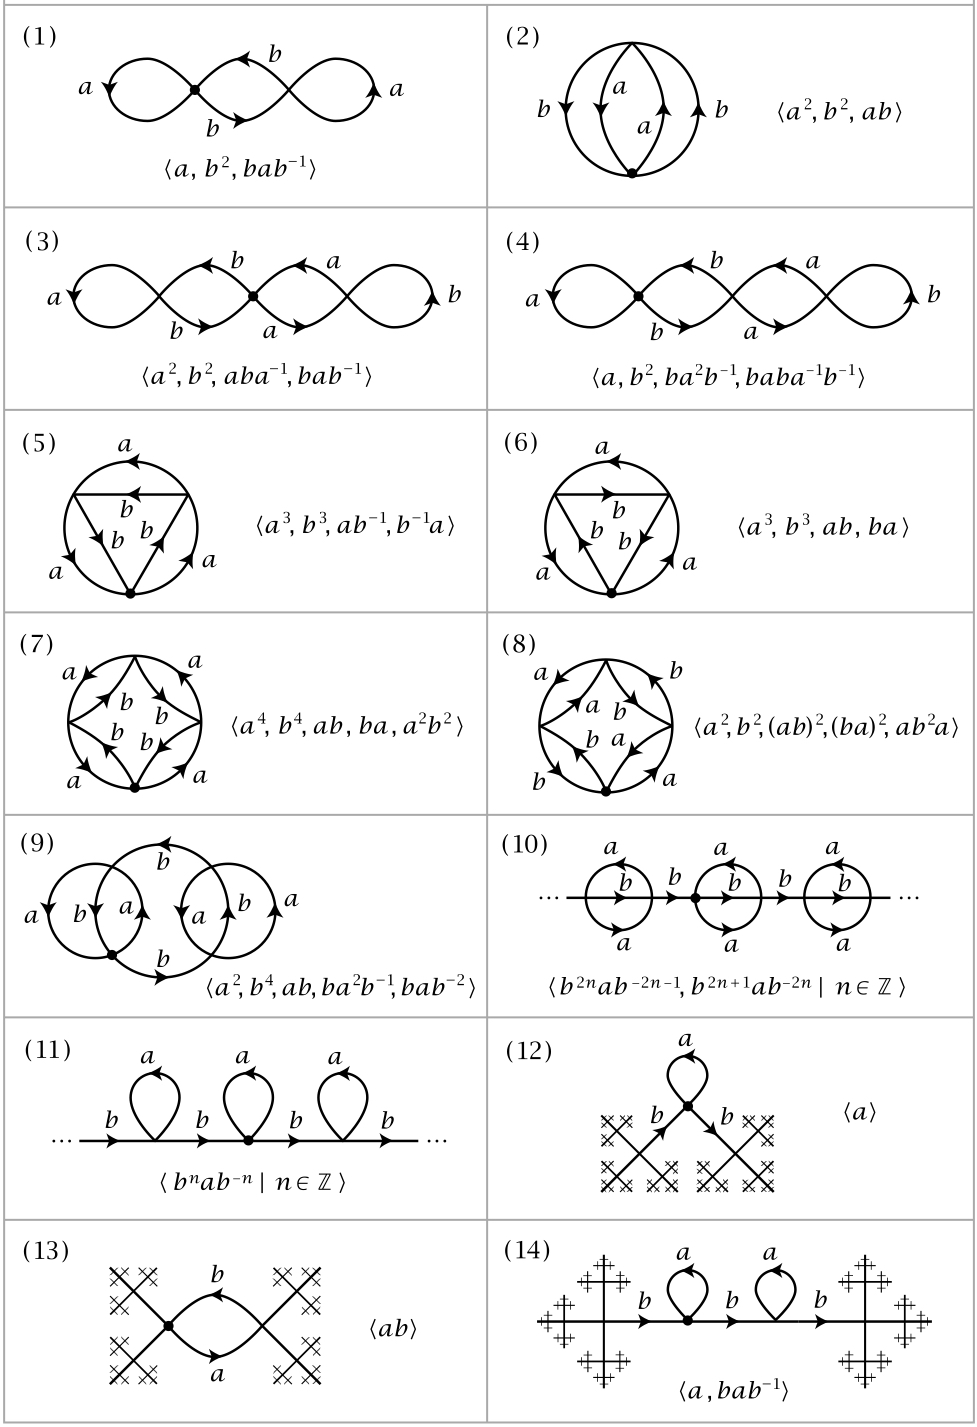
\includegraphics[width=\textwidth]{coveringsOfS1S1.jpg}
  \caption*{Coverings of $S^1 \vee S^1$. Image from Algebraic Topology, Allen Hatcher, Chapter 1.}
  % \label{fig:CoveringsOfS1S1}
\end{figure}

  \section{Galois correspondence of covering spaces}
For this section, fix a Galois cover $p: Y \longrightarrow X$.

\begin{lemma}
\label{lemma:compositionOfCovers}
  If $p$ factors through a space $Z$ as
  \begin{equation*}
    \begin{tikzcd}
      Y \ar[rd, "p_1"] \ar[dd, "p"']\\
        & Z \ar[ld,"p_2"] \\
      X
    \end{tikzcd}
  \end{equation*}
  and if $p_2$ is a cover, then so is $p_1$.
  In this case, we say that $Z$ is a cover \emph{lying between $Y$ and $X$.}
\end{lemma}
\begin{qbox}
  Prove Lemma \ref{lemma:compositionOfCovers} by drawing pictures.
\end{qbox}

\begin{lemma}
\label{lemma:lemma2}
  If $p_2:Z \rightarrow X$ be a cover. Let $f$, $g$ be simplicial maps $Y \rightarrow Z$ that fit into a commutative diagram
  \begin{equation*}
    \begin{tikzcd}
      Y \ar[rr, shift left, "f"] \ar[rr, shift right, "g"']  \ar[rd, "p"']
      & & Z \ar[ld,"p_2"] \\
      & X
    \end{tikzcd}
  \end{equation*}
  If $f(y_0) = g(y_0)$ for some vertex $y_0$ in $Y$ then $f = g$.
\end{lemma}
\begin{qbox}
  Prove Lemma \ref{lemma:lemma2} for vertices i.e. show that $f(y) = g(y)$ for all vertices $y$ in $Y$. To do this, take a path $\gamma$ in $Y$ from $y_0$ to $y$, push it down to $X$ via $p$ and lift it up to $Z$ via $p_2$. Use induction on the length of $\gamma$.
\end{qbox}


\begin{proposition}
  If $Z$ is a cover lying between $Y$ and $X$, then $p_1: Y \rightarrow Z$ is a Galois cover.
\end{proposition}
\begin{proof}
  We have already shown that $p_1$ is a cover in Lemma \ref{lemma:compositionOfCovers}.
  In order to show that it is Galois we will use the criterion of Theorem \ref{theorem:GaloisCriterion}:
  ``$p_1$ is Galois if and only if $\Gal(Y|Z)$ acts freely, transitively on all the fibers.''
  First note that every deck transformation of $Y \rightarrow Z$ is also a deck transformation of $Y \rightarrow X$
  \begin{equation*}
    \begin{tikzcd}
      Y \ar[rr, "\varphi"] \ar[rd, "p_2"] \ar[rdd, "p"']
      & & Y \ar[ld,"p_2"'] \ar[ldd, "p"]\\
      & Z \ar[d] \\
      & X
    \end{tikzcd}
  \end{equation*}
  Hence $\Gal(Y|Z)$ is a subgroup of $\Gal(Y|X)$.
  We want to show that $\Gal(Y|Z)$ acts freely, transitively on the fibers $p_2^{-1}(Z)$.
  The freeness is by Theorem \ref{theorem:freenessGaloisAction} so we only need to prove transitivity.

  Pick an arbitrary element $z$ in $Z$ and let $y_1$ and $y_2$ be elements in the fiber $p_2^{-1}(z)$.
  As $Y \rightarrow X$ is Galois, there is a deck transformation $\varphi \in \Gal(Y|X)$ such that $\varphi(y_1) = y_2$.

  \textbf{Claim:} $\varphi$ is in $\Gal(Y|Z)$.

  To prove this claim, apply Lemma \ref{lemma:lemma2} to the following commutative diagram
  \begin{equation*}
    \begin{tikzcd}
      Y \ar[rr, shift left, "p_1"] \ar[rr, shift right, "p_1 \circ \varphi"']  \ar[rd, "p"']
      & & Z \ar[ld,"p_2"] \\
      & X
    \end{tikzcd}
  \end{equation*}
  Check that we can apply lemma 2: 1) $\varphi$ is a deck transformation of $p$, hence the diagram commutes. 2) $p_1(y_1) = p_1 \circ \varphi(y_1) = z$.
  By Lemma \ref{lemma:lemma2}, $p_1 = p_1 \circ \varphi$ i.e. $\varphi$ is a deck transformation in $\Gal(Y|Z)$.
  Hence, the action of $\Gal(Y|Z)$ on the fibers of $p_2$ is transitive.
\end{proof}

\begin{proposition}
  If $Z$ is a cover lying between $Y$ and $X$, and $p_2:Z \rightarrow X$ is Galois, then $\Gal(Y|Z)$ is a normal subgroup of $\Gal(Y|X)$, and\footnote{This is equivalent to saying that the following sequence is exact. \begin{equation*}
    1 \rightarrow \Gal(Y|Z) \rightarrow \Gal(Y|X) \rightarrow \Gal(Z|X) \rightarrow 1
  \end{equation*}}
    \begin{align*}
      \Gal(Z|X) \cong \Gal(Y|X) / \Gal(Y|Z).
    \end{align*}
\end{proposition}
\begin{proof}
  Let $\varphi \in G$ be a deck transformation in $\Gal(Y|X)$. We will first show that $\varphi$ descends to a deck transformation in $\Gal(Z|X)$ i.e. there is a $\psi$ that fits in the commutative diagram
  \begin{equation*}
    \begin{tikzcd}
      Y \ar[rrrr, "\varphi"] \ar[rd, "p_1"']
      & & & &
      Y  \ar[ld, "p_1"]\\
      & Z \ar[rr, shift left, "\psi"] \ar[rd,"p_2"']
      & & Z \ar[ld,"p_2"] \\
      & &  X
    \end{tikzcd}
  \end{equation*}
  To do this, pick an element $y \in Y$ and let $ z = p_1(y)$.
  Because $Z \rightarrow X$ is Galois, there is a unique deck transformation $\psi \in \Gal(Z|X)$ which sends $p_1(y)$ to $p_1(\varphi(y))$.
  We need to show that $p_1 \circ \varphi = \psi \circ p_1$.
  For this, apply Lemma \ref{lemma:lemma2} to the following commutative diagram
  \begin{equation*}
    \begin{tikzcd}
      Y \ar[rr, shift left, "\psi \circ p_1"] \ar[rr, shift right, "p_1 \circ \varphi"']  \ar[rd, "p"']
      & & Z \ar[ld,"p_2"] \\
      & X
    \end{tikzcd}
  \end{equation*}
  \begin{qbox}
    Finish the above argument. Then show that $\varphi \mapsto \psi$ defines a group homomorphsism $\Gal(Y|X) \rightarrow \Gal(Z|X)$ with kernel $\Gal(Y|Z)$ thereby completing the proof.
  \end{qbox}
\end{proof}





\begin{proposition}
  If $Z$ is a cover lying between $Y$ and $X$ and $\Gal(Y|Z)$ is a normal subgroup of $\Gal(Y|X)$, then $p_2:Z \rightarrow X$ is Galois.
\end{proposition}
  \begin{qbox}
    Using $Z \cong Y/H$, $X \cong Y/G$, argue that $X \cong Z/(G/H)$. Use this to prove the Proposition.
  \end{qbox}





\begin{theorem}[Galois Correspondence of Covering Spaces]
  There is a 1-1 correspondence between the subgroups of $\Gal(Y|X)$ and covers of $X$ that lie between $Y$ and $X$, given by the following maps
  \begin{align*}
    \{\mbox{ subgroups of $\Gal(Y|X)$ } \} &\longleftrightarrow  \{\mbox{ covers lying between $Y$ and $X$ } \}\\
    H &\longmapsto Y/H \\
    \Gal(Y|Z) & \longmapsfrom Z
  \end{align*}
  Under this correspondence, the normal subgroups of $\Gal(X|Y)$ correspond to Galois covers of $X$.
\end{theorem}
\begin{qbox}
  We have proved all the parts of this theorem. Write down the proof explicitly and see how the various pieces fit together.
\end{qbox}

\begin{remark}
  There is a subtle point here about what the correspondence is between. On the right hand side, the objects are not spaces $Z$ but the triangles of the form \begin{equation*}
    \begin{tikzcd}
      Y \ar[rd, "p_1"] \ar[dd, "p"']\\
        & Z \ar[ld,"p_2"] \\
      X
    \end{tikzcd}
  \end{equation*}
\end{remark}


\begin{qbox}
  Explicitly right down the Galois correspondence for
  \begin{enumerate}
    \item The covers of $S^1 \vee S^1$ in Figure \ref{fig:CoveringsOfS1S1}.
    \item The cover $\bbr^1 \rightarrow S^1$.
  \end{enumerate}
\end{qbox}










\iffalse
\section*{Review the following for tomorrow}
For tomorrow's class, please review/lookup \emph{presentation of a group}. The following statements should make sense to you
\begin{align*}
  \bbz &= \langle a \rangle \\
  \bbz/n &= \langle a | a^n \rangle \\
  \bbz \times \bbz &= \langle a, b | ab a^{-1} b^{-1} \rangle \\
  D_{2n} &= \langle r, s | r^n, s^2, (rs)^2 \rangle && \mbox{ where $D_{2n}$ is the Dihedral group.}
\end{align*}








\section{Lifting properties of covering spaces}


We have a complete description of what the covers lying between $X$ and $Y$ are.

\begin{theorem}
  \label{theorem:liftingOfCovers}
  Consider covering maps
  \begin{equation*}
    \begin{tikzcd}
      & X \ar[d,"p"] \\
      Z \ar[r, "p'"']& Y
    \end{tikzcd}
  \end{equation*}
  along with vertices $x \in X, y \in Y, z \in Z$ with $p(x) = z = p'(y)$. There exists a map $p'':Z \rightarrow X$ which factors $p'$ with $p'(z) = y$ if and only if
  \begin{align*}
    p'_*\pi_1(Z,z) \le p_* \pi_1(X,x).
  \end{align*}
  In this case, the lift $p''$ is unique.
\end{theorem}

  \begin{corollary}
    A simply connected space has no non-trivial (connected) covers.
  \end{corollary}

  A map between spaces $p:X \rightarrow Y$ naturally induces a map between fundamental groups
  \begin{equation*}
    p_*: \pi_1(X,x) \rightarrow \pi_1(Y,y)
  \end{equation*}

  \fi

  \section{Fundamental group and monodromy action}
Fix a space $X$ and a vertex $x$ on it.

Recall that, a \emph{path} $\gamma$ in $X$ is a finite sequence of edges $e_1 e_2 e_3 \dots e_k$, where we allow inverses, such that $d_1 e_i = d_0 e_{i+1}$ for $1 \le i \le k-1$.
Denote $d_0 \gamma = d_0 e_1$ and $d_1 \gamma = d_1 e_k$.

We can concatenate two paths $\gamma_1$, $\gamma_2$ if $d_1 \gamma_1 = d_0 \gamma_2$ to get a path $\gamma_1 \cdot \gamma_2$ from $d_0 \gamma_1$ to $d_1 \gamma_2$.
For a vertex $x \in X$, we denote by $\mathbb{1}_x$ the path of length 0 starting at $x$, with the property that $d_0 \mathbb{1}_x = x = d_1 \mathbb{1}_x$ and $\gamma \cdot \mathbb{1}_x = \gamma$ and $ \mathbb{1}_x \cdot \gamma = \gamma$ whenever the concatenations make sense.

A \emph{loop} at $x$ is a path starting and ending at $x$. Concatenation defines a product on the set of loops.

The \emph{fundamental group} of $X$ at $x$ is essentially
\begin{equation*}
  \pi_1(X,x) = \langle \mbox{ loops } | \mbox{ faces }\rangle
\end{equation*}
There are multiple ways to make this definition precise. We will do this recursively.

We add \emph{generators} using edges.
\begin{enumerate}
  \item Start with just the vertex $x$.
  \item Add edges successive (while keeping the space connected).
  \item Every time the newly added edge $e$ forms a loop $\gamma$, add $\gamma$ as a generator to $\pi(X,x)$.
\end{enumerate}

We add \emph{relations} using faces.
\begin{enumerate}
  \item Add the faces one at a time.
  \item For each face, let $\gamma'$ be the boundary of the face starting at $y$.
  \item Add the relation $\gamma \cdot \gamma' \cdot \gamma^{-1}$ to $\pi_1(X,x)$ where $\gamma$ is a path connecting $x$ to $y$.
\end{enumerate}

\begin{remark}
  If you think that this definition is artificial and contrived, then you are correct. There is a very natural object called the \emph{fundamental groupoid} associated to the space $X$ which does not depend on the basepoint $x$.
\end{remark}


  \begin{ex}
    The fundamental group of $S^1$ has a single generator and there are no relations.
    Hence,
    \begin{align*}
      \pi_1(S^1) = \langle a \rangle \cong \bbz
    \end{align*}
    \begin{figure}[H]
    \centering
      % \includegraphics[width=0.5\textwidth]{example-image}
      \begin{tikzpicture}[scale=0.5]
        \filldraw (0,0) circle (2pt);
\draw [->] (0,0) to [bend left=45] (1,1)  to [bend left=45] (2,0) node [right] {$a$};
\draw (2,0) to [bend left=45] (1,-1)  node [below] {$S^1$} to [bend left=45] (0,0);

      \end{tikzpicture}
      \caption{Fundamental group of a circle is $\bbz$.}
    \end{figure}
  \end{ex}

  \begin{ex}
    The fundamental group of $S^1 \vee S^1$ has a single generator and there are no relations.
    Hence,
    \begin{align*}
      \pi_1(S^1 \vee S^1) = \langle a, b \rangle \cong F_2
    \end{align*}
    which is the free group on two generators.
    \begin{figure}[H]
    \centering
      % \includegraphics[width=0.5\textwidth]{example-image}
      \begin{tikzpicture}[scale=0.5]
        \filldraw (0,0) circle (2.5pt);

\draw [->] (0,0) to [bend right=45] (-1,1) to [bend right=45] (-2,0) node [left] {$a$} ;
\draw (-2,0) to [bend right=45] (-1,-1) to [bend right=45] (0,0);

\draw [->] (0,0) to [bend right=45] (1,-1) to [bend right=45] (2,0) node [right] {$b$};
\draw (2,0) to [bend right=45] (1,1) to [bend right=45] (0,0);

      \end{tikzpicture}
      \caption{Fundamental group of $S^1 \vee S^1$ is $\bbz$.}
    \end{figure}
  \end{ex}

  \begin{ex}
    The fundamental group on cylinder is given by
    \begin{align*}
      \pi_1(\mbox{cylinder})
      &= \langle c, a b a^{-1} \mid  a b a^{-1} c\rangle \\
      &= \langle c \rangle \\
      &\cong \bbz
    \end{align*}
  \end{ex}

    \begin{ex}
      The fundamental group on torus is given by
      \begin{align*}
        \pi_1(\mbox{torus})
        &= \langle a, b \mid a b a^{-1} b^{-1} \rangle \\
        &\cong \bbz \times \bbz
      \end{align*}
    \end{ex}

  \begin{qbox}
    Find the fundamental groups of
    \begin{enumerate}
      \item $S^2$
      \item Mobius strip
      \item Klein bottle
      \item Real projective space
    \end{enumerate}
  \end{qbox}

  \begin{proposition}
    For any two vertices $x_1$, $x_2 \in X$ there exists an isomorphism
    \begin{equation*}
      \pi_1(X,x_1) \xrightarrow{\cong} \pi_1(X,x_2).
    \end{equation*}
  Henc, the fundamental group does not depend on the basepoint upto isomorphism.
\end{proposition}
  \begin{qbox}
    Pick a path $\gamma \in X$ from $x$ to $x'$.
    Conjugate by $\gamma$ to get an isomorphism between $\pi_1(X,x)$ and $\pi_1(X,x')$.
  \end{qbox}

\subsection{Monodromy}
\begin{proposition}
  A covering map $p:Y \rightarrow X$ induces a group homomorphism
  \begin{align*}
    p_* : \pi_1(Y,y) &\longrightarrow \pi_1(X,x), \\
    [\gamma] &\longmapsto [p(\gamma)].
  \end{align*}
  where $x = p(y)$.
  If $p$ is a non-trivial cover then $p_*$ is strictly injective i.e. $p_*\pi_1(Y,y)$ is a proper subgroup of $\pi_1(X,x)$.
\end{proposition}
\begin{proof}
  The group homomorphism is evident as $p$ preserves concatenation of paths.

  For injectivity, suppose $[p(\gamma)]$ is trivial inside $\pi_1(X,x)$.
  This means that $p(\gamma)$ is a product of terms of the form $\gamma \cdot \gamma' \cdot \gamma^{-1}$ where $\gamma'$ is the boundary of a face. Hence, $\gamma$ is a product of the lifts $\widetilde{\gamma} \cdot \widetilde{\gamma}' \cdot \widetilde{\gamma}^{-1}$.
  But $\widetilde{\gamma}'$ is also the boundary of a face as $p$ is a simplicial map.
  Hence, $[{\gamma}]$ is trivial $\implies$ $p_*$ is injective.

  $p_*$ is strictly injective as a path $y_1$ to $y_2$, both in the fiber over $x$, map down to a loop at $x$, say $\gamma$.
  By uniqueness of path lifting, there is no path that maps down to $\gamma$.
\end{proof}

\begin{theorem}
  Let $p:Y \rightarrow X$ be a Galois cover. Let $y$ be a vertex in $Y$ in the fiber over the vertex $x$ in $X$.
  Then there is a surjective group homomorphism
  \begin{align*}
    M:\pi_1(X,x) \longrightarrow \Gal(Y|X)
  \end{align*}
  whose kernel is $p_*(\pi_1(Y,y))$.
  We say that the loops in $X$ act via ``monodromy'' on the space $Y$.
\end{theorem}
\begin{proof}
  The map $M$ is defined as follows.
  Let $y$ be a point $y$ in the fiber over $x$ and let $\gamma$ be a loop in the base starting at $x$.
  Consider the unique lift $\widetilde{\gamma}$ starting at $y$.
  Because $p:Y \rightarrow X$ is Galois, there is a unique deck transformation $\varphi_{\gamma} \in \Gal(Y|X)$ sending $y$ to $d_1 \widetilde{\gamma}$.
  Then define
  \begin{equation*}
    M(\gamma) = \varphi_{\gamma}
  \end{equation*}
  In order to show that this map descends to $\pi_1(X,x)$ we need to show that $\gamma \cdot \gamma' \cdot \gamma^{-1}$ gets mapped to the trivial deck transformation, where $\gamma'$ is the boundary of a face.
  \begin{qbox}
    Check this.
  \end{qbox}

  The kernel of $M$ is the set of loops which lift to loops at $y$, which is the same as the set of loops in $X$ which are images of loops in $Y$, but this is precisely $p_*(\pi_1(Y,y))$.

  It remains to show that $M$ is a group homomorphism.
  Let $\gamma_1$ and $\gamma_2$ be two loops in $\pi_1(X,x)$. Suppose $d_1 \widetilde{\gamma_1} = y_1$ and $d_1 \widetilde{\gamma_2} = y_2$. Let $\varphi_1 = M \gamma_1$ and $\varphi_2 = M \gamma_2$ so that $ \varphi_1(y) = y_1$ and $\varphi_2(y) = y_2$.
  By unique path lifting it follows that the lift of $\widetilde{\gamma_1 \cdot \gamma}$ is the path that ends in $\varphi_1(y_2) = \varphi_1 \varphi_2 y$.
  Hence, $M$ sends $\gamma_1 \cdot \gamma_2$ to $\varphi_1 \cdot \varphi_2$.
\end{proof}


\begin{theorem}
  \label{theorem:fundamentalGroupQuotient}
  We can rewrite the above theorem as saying that if $p:Y \rightarrow X$ is a Galois cover with $p(y) = x$, then there is a short exact sequence of groups
  \begin{equation*}
    1 \rightarrow \pi_1(Y,y) \xrightarrow{p_*} \pi_1(X,x) \rightarrow \Gal(Y|X) \rightarrow 1
  \end{equation*}
\end{theorem}

\begin{qbox}
  Verify Theorem \ref{theorem:fundamentalGroupQuotient} for the coverings $(1)$, $(2)$, $(6)$, and $(11)$ of $S^1 \vee S^1$ in Figure \ref{fig:CoveringsOfS1S1}.
\end{qbox}

\begin{qbox}
  Verify Theorem \ref{theorem:fundamentalGroupQuotient} for the coverings
  \begin{align*}
    \mbox{Cylinder} &\longrightarrow \mbox{Mobius Strip} \\
    \mbox{Torus} &\longrightarrow \mbox{Klein Bottle} \\
    \mbox{Sphere } S^2 &\longrightarrow \mbox{Real projective space}
  \end{align*}
\end{qbox}







\begin{figure}[p]
\centering
  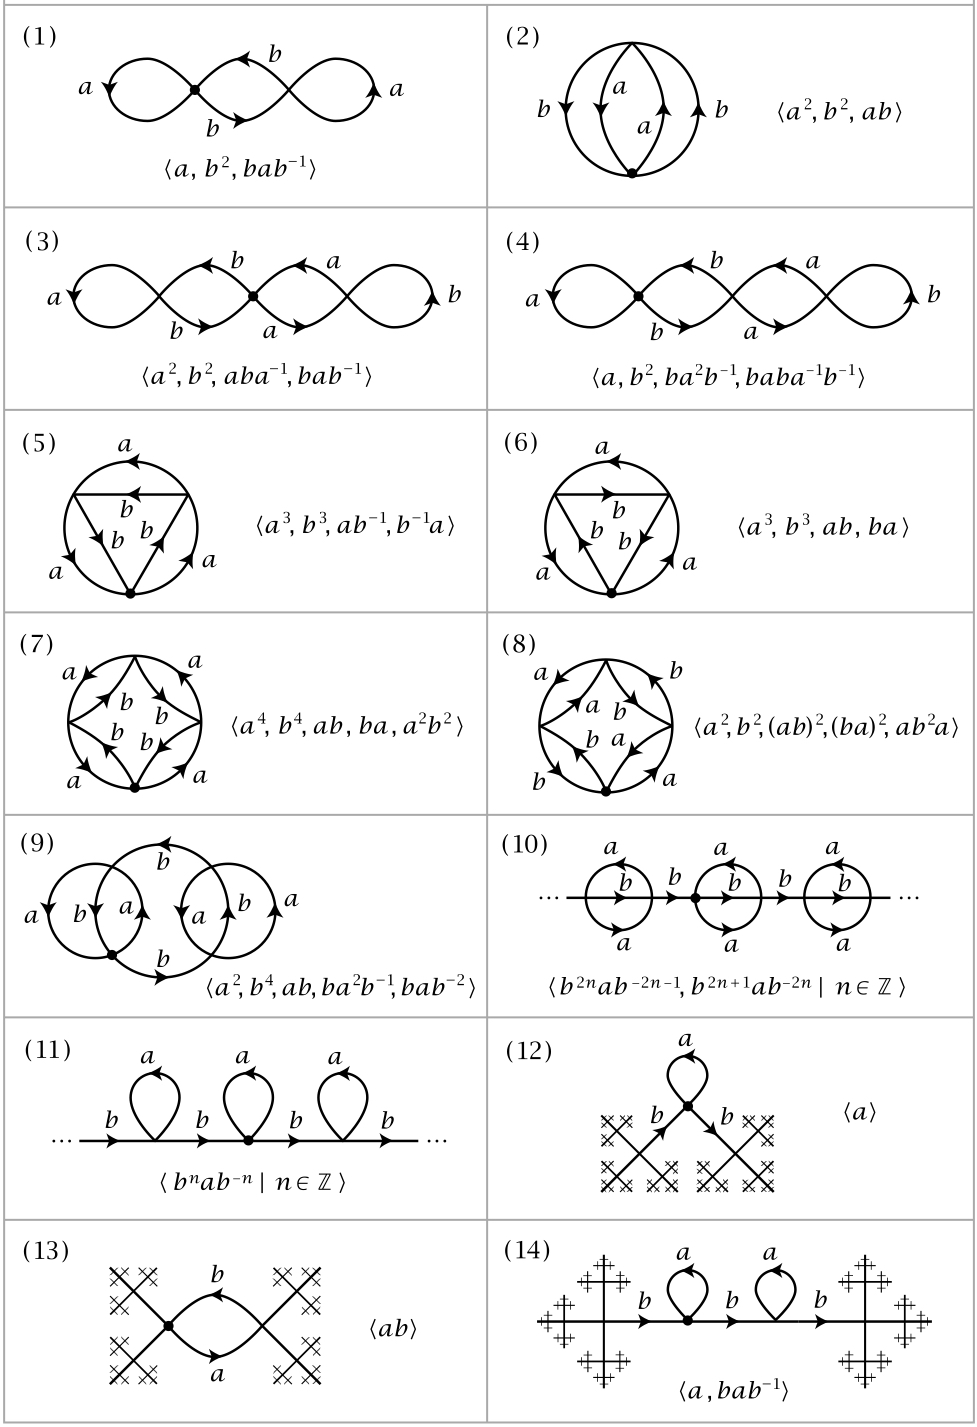
\includegraphics[width=\textwidth]{coveringsOfS1S1.jpg}
  \caption*{Coverings of $S^1 \vee S^1$. Image from Algebraic Topology, Allen Hatcher, Chapter 1.}
\end{figure}

\begin{figure}[p]
  \centering
  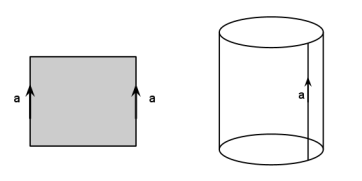
\includegraphics[width=0.65\textwidth]{cylinderGluingDiagram.png}
  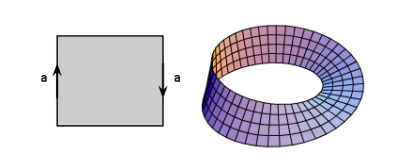
\includegraphics[width=0.65\textwidth]{MobiusStripGluingDiagram.png}

  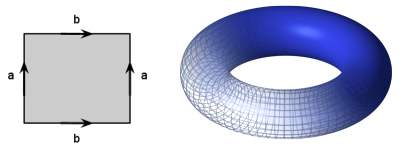
\includegraphics[width=0.65\textwidth]{torusGluingDiagram.png}
  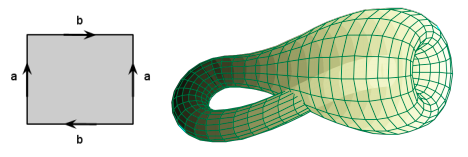
\includegraphics[width=0.65\textwidth]{KleinBottleGluingDiagram.png}

  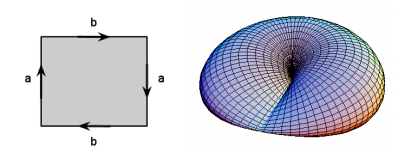
\includegraphics[width=0.65\textwidth]{RP2GluingDiagram.png}
  \caption*{Gluing diagrams for cylinder, Mobius strip, torus, Klein bottle, real projective space respectively. Images from BMC Notes on Surfaces by Maia Averett.}
\end{figure}

  \section{Universal cover}

The following two theorems summarize our results about covering spaces.

\begin{theorem}[Galois Correspondence of Covering Spaces]
  There is a 1-1 correspondence between the subgroups of $\Gal(Y|X)$ and covers of $X$ that lie between $Y$ and $X$, given by the following maps
  \begin{align*}
    \{\mbox{ subgroups of $\Gal(Y|X)$ } \} &\longleftrightarrow  \{\mbox{ covers lying between $Y$ and $X$ } \}\\
    H &\longmapsto Y/H \\
    \Gal(Y|Z) & \longmapsfrom Z
  \end{align*}
  Under this correspondence, the normal subgroups of $\Gal(X|Y)$ correspond to Galois covers of $X$.
\end{theorem}

\begin{theorem}[Monodromy action of the fundamental group]
  \label{theorem:fundamentalGroupQuotient2}
  If $p:Y \rightarrow X$ is a Galois cover with $p(y) = x$, then there is a short exact sequence of groups
  \begin{equation*}
    \begin{tikzcd}
      1 \ar[r] & \pi_1(Y,y) \ar[r, "p_*"] & \pi_1(X,x) \ar[r,"M"] &  \Gal(Y|X) \ar[r] & 1
    \end{tikzcd}
  \end{equation*}
  where the map $p_*$ is sending a loop $\gamma$ in $Y$ to $p(\gamma)$ and $M$ is the monodromy action.
\end{theorem}

We will assume the following for now without proof.
\begin{theorem}[Existence of universal cover]
  For any space $X$, there exists a space $\widetilde{X}$ with a covering map $P:\widetilde{X} \rightarrow X$ satisfying the following properties:
  \begin{enumerate}
    \item $P$ is Galois.
    \item $\pi_1(\widetilde{X})$ is trivial. (We say that $\widetilde{X}$ is simply connected.)
    \item Every cover $Y$ of $X$ lies between $\widetilde{X}$ and $X$.
  \end{enumerate}
  Such a space $\widetilde{X}$ is called the \emph{universal cover} of $X$.
\end{theorem}

Several corrolaries follow immediately from this statement.












\subsection{Classification of all covers}



\begin{proposition}
  $\Gal(\widetilde{X} | X) \cong \pi_1(X,x)$.
\end{proposition}
\begin{proof}
  Apply Theorem \ref{theorem:fundamentalGroupQuotient2} to the cover $P:\widetilde{X} \rightarrow X$.
\end{proof}

\begin{theorem}[Galois correspondence \#2]
  \label{theorem:GaloisCorrespondence2}
  There is a 1-1 correspondence between the subgroups of $\pi_1(X,x)$ and covers of $X$, given by the following maps
  \begin{align*}
    \{\mbox{ subgroups of $\pi_1(X,x)$ } \} &\longleftrightarrow  \{\mbox{ covers of $X$ } \}\\
    H &\longmapsto \widetilde{X}/H \\
    \pi_1(Z,z) & \longmapsfrom Z
  \end{align*}
  Under this correspondence, the normal subgroups of $\pi_1(X,x)$ correspond to Galois covers of $X$.
\end{theorem}






\subsection{Subgroups of a free group}
Denote by $F_n$ the free group with $n$ generators.
\begin{theorem}
  Every subgroup of a finitely generated free group is free.
\end{theorem}
\begin{proof}
  Let $G = \mathrm{Free}(S)$ be a finitely generated free group with $|S|=k$.
  Let $X$ be a wedge of $k$ circles, so that $\pi_1(X) = G$.
  \begin{figure}[H]
    \centering
    \begin{tikzpicture}[scale=0.5]
     \begin{polaraxis}[grid=none, axis lines=none]
  \addplot[mark=none,domain=0:360,samples=300] {cos(x*5)};
\end{polaraxis}

    \end{tikzpicture}
    \caption{Wedge of 5 circles $\bigvee \limits_5 S^1$ has fundamental group $F_5$.}
  \end{figure}
  Every cover of $X$ is a graph, and the fundamental group of a graph is a free group (as there are no faces).
  Hence, by Theorem \ref{theorem:GaloisCorrespondence2} every subgroup of $G$ is free.
\end{proof}







\begin{theorem}
  If $F_m \triangleleft F_n$ then $n - 1 | m - 1$ and the index of $F_m$ inside $F_n$ is $(m-1)/(n-1)$.
\end{theorem}
\begin{proof}
  A normal subgroup $H$ of $G$ corresponds to a Galois cover $X$ of $\bigvee \limits_n S^1$, of some degree, say $d$.
  As $X$ is a cover, one can check by simple edge conting, that $X$ is free group on $(n-1)d + 1$ generators.
  The result follows.
\end{proof}









\subsection{Universal property of the universal cover}

We say that a space $Y$ is simply connected if $\pi_1(Y) \cong \set{\mathbb{1}}$.
\begin{proposition}
  Let $p:Y \rightarrow X$ be a Galois cover such that $Y$ is simply-connected.
  Further suppose that $p_2:Z \rightarrow X$ is another cover then $Z$ is a subcover of $Y$.
  \begin{equation*}
    \begin{tikzcd}
      Y \ar[rd, dashed, "\exists"] \ar[dd, "p"']\\
        & Z \ar[ld,"p_2"] \\
      X
    \end{tikzcd}
  \end{equation*}
\end{proposition}
\begin{proof}
  We will explicitly construct a map $p_1: Y \rightarrow Z$.
  Pick vertices $y_0$ in $Y$, $x_0$ in $X$, and $z_0$ in $Z$ such that $p(y_0) = x_0 = p_2(z_0)$.
  We define $p_1(y_0) = z_0$.

  Let $y$ be a vertex in $Y$. Let $\gamma$ be a path in $Y$.
  We push down $\gamma$ to X then lift it up to $X$ and set $p_1(y) = d_1 \widetilde{p(\gamma)}$.
  \begin{equation*}
    \begin{tikzcd}
      \gamma \ar[dd, mapsto]\\
        & \widetilde{p(\gamma)}  \\
      p(\gamma) \ar[ur, mapsto]
    \end{tikzcd}
  \end{equation*}

  We need to check that the map defined this way is well-defined i.e. it does not depend on the choice of the path $\gamma$.
  Suppose there are two paths $\gamma_1$ and $\gamma_2$ connecting $y_0$ to $y$.
  Then $\gamma_1^{-1} \gamma_2$ is a loop at $y$ and hence is (upto conjugation) a boundary of a face.
  It follows from this that the lifts of both $\gamma_1$ and $\gamma_2$ have the same endpoints.
\end{proof}


And so a universal cover of $X$ is any cover $\widetilde{X}$ of $X$ that is simply-connected.
There is a theorem of existence of the universal space of a general space, but in practice we simply construct these spaces by hand.

\begin{ex}
  The universal cover of $S^1$ is $\bbr^1$.
\end{ex}

\begin{ex}
  The universal cover of a cylinder (and hence also a Mobius strip) is $\bbr^1 \times [0,1]$.
\end{ex}

\begin{ex}
  The universal cover of a torus (and hence also a Klein bottle) is $\bbr^2$.
\end{ex}

\begin{ex}
  The universal cover of a real projective space is $S^2$.
\end{ex}

\begin{ex}
  The universal cover of a bouquet of $k$ circles is the Cayley graph of the free group with $k$ generators.
  \begin{figure}[H]
  \centering
    % \includegraphics[width=0.5\textwidth]{example-image}
    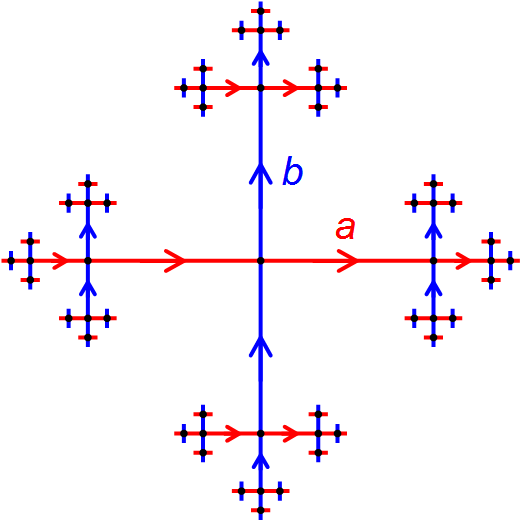
\includegraphics[width=0.5\textwidth]{CayleyF2.png}
    \caption{Universal cover of $F_2$}
  \end{figure}
\end{ex}

\begin{ex}
  A universal cover of a graph $X$ (space with no faces) can be constructed as follows:
  \begin{enumerate}
    \item Pick a vertex $x$.
    \item $\widetilde{X}$ is a graph whose vertices are paths in $X$ that start at $x$.
    \item There is an edge from $\gamma$ and $\gamma'$ if $\gamma = \gamma' \cdot e$ for some edge $e$.
    \item The covering map $P:\widetilde{X} \rightarrow X$ is the map $\gamma \mapsto d_1 \gamma$.
  \end{enumerate}
  \begin{qbox}
    Show that the $\widetilde{X}$ defined above is a simply-connected space and that $P$ is a covering map, and hence $\widetilde{X}$ is a universal cover.
  \end{qbox}
  This method can be generalized to spaces with faces. In this case, instead of taking all paths we need to take equivalence classes of paths with respect to boundaries of faces.
  \begin{equation*}
    \widetilde{X}_x = \set{ \mbox{paths starting at } x} / \mbox{faces}
  \end{equation*}
\end{ex}

\begin{remark}
  Finally, here is a comparison of the Galois correspondences for algebra and topology from Terrence Tao's blog \cite{TerrenceTao}.
  \begin{figure}[H]
  \centering
    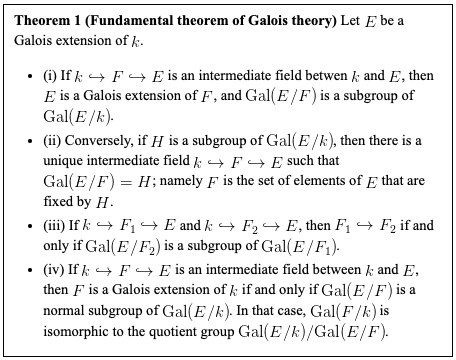
\includegraphics[width=0.8\textwidth]{TerryTao1.png}
    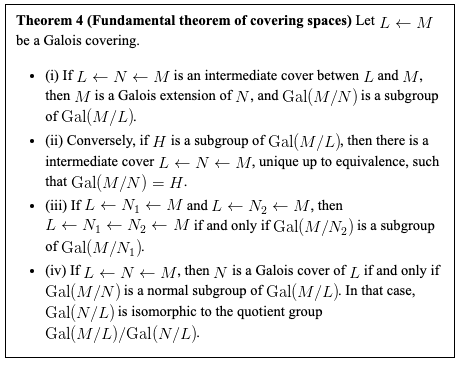
\includegraphics[width=0.8\textwidth]{TerryTao2.png}
  \end{figure}

\end{remark}

\begin{thebibliography}{9}
\bibitem{Szamuely}
Tam\'as Szamuely, \emph{Galois Groups and Fundamental Groups}, Cambridge Studies in Advanced Mathematics, 2007.

\bibitem{TerrenceTao}
Terrence Tao, \emph{Trying to understand the Galois correspondence},\\ \url{https://terrytao.wordpress.com/2018/08/28/trying-to-understand-the-galois-correspondence/}.
\end{thebibliography}


% In this section, we'll prove that for every (connected) space $Y$ and a vertex $y \in Y$, there exists a simply-connected space $\widetilde{Y}_y$ with a covering map
% \begin{align*}
%   \widetilde{Y}_y \rightarrow Y
% \end{align*}
%
% By Theorem \ref{theorem:liftingOfCovers} this cover is universal, in the sense that every cover $Z \rightarrow Y$ lies between $\widetilde{Y}_y$ and $Y$.
% \begin{equation*}
%   \begin{tikzcd}
%     & Z \ar[d] \\
%     \widetilde{Y}_y \ar[ur,"\exists !",dashrightarrow] \ar[r, "p'"']& Y
%   \end{tikzcd}
% \end{equation*}
%
% The following lemmas are more or less true by definition.
% \begin{lemma}
%   The fundamental group of a graph (=space with only vertices and edges) is a free group.
% \end{lemma}
%
% \begin{lemma}
%   Every cover of a graph is a graph.
% \end{lemma}

\end{document}
